\begin{frame}{Galat pemotongan (\textit{truncation error})}

Galat pemotongan adalah galat yang dihasilkan karena penggunaan
suatu aproksimasi dibandingkan dengan prosedur eksak.

Contohnya adalah penggunaan persamaan beda hingga untuk mengaproksimasi
turunan pertama:
$$
\frac{\partial v}{\partial t} \approx \frac{\Delta v}{\Delta t}
= \frac{v(t_{i+1}) - v(t_{i})}{t_{i+1} - t_{i}}
$$
Galat yang terjadi akibat penggunaan rumus ini adalah galat pemotongan
karena rumus ini hanya memberikan aproksimasi dari nilai turunan sebenarnya.

Galat pemotongan dapat muncul dalam berbagai konteks. Kita akan melihat galat
pemotongan dari sudut pandang ekspansi deret Taylor.

\end{frame}



\begin{frame}{Deret Taylor}

Deret Taylor dapat digunakan untuk menghitung nilai
fungsi $f(x)$ di suatu titik $x_{i+1}$ dengan informasi atau input
nilai fungsi dan turunan-turunannya pada suatu titik referensi $x_{i}$.

Deret Taylor dapat dituliskan sebagai:
\begin{equation}
f(x_{i+1}) = f(x_i) + f'(x_{i}) + \frac{f''(x_i)}{2!}h^2 + \cdots +
\frac{f^{(n)}(x_i)}{n!}h^n + R_{n}
\end{equation}
dengan $R_{n}$ adalah suku sisa:
\begin{equation}
R_{n} = \frac{f^{(n+1)}(\xi)}{(n+1)!}h^{n+1}
\end{equation}
di mana $\xi$ adalah suatu bilangan yang terletak pada pada selang
$[x_i, x_{i+1}]$.

\end{frame}


\begin{frame}

\fontsize{9}{10}\selectfont

\begin{block}{Chapra Contoh 4.1}
Gunakan ekspansi deret Taylor untuk mengaproksimasi fungsi:
$$
f(x) = -0.1 x^{4} - 0.15 x^{3} - 0.5 x^{2} - 0.25 x + 1.2
$$
di sekitar $x_{i} = 0$ dengan $h=1$ (artinya kita diminta untuk menentukan
aproksimasi dari fungsi pada saat $x_{i+1}=1$). Hitung juga galat pemotongan
yang terjadi.
\end{block}

Pada contoh ini fungsi $f(x)$ diketahui, sehingga kita dapat menggunakan
ekspresi dari $f(x)$ secara langsung untuk mengetahui nilai dari $f(x=1)$
tanpa menggunakan deret Taylor.
Tujuan dari latihan ini adalah untuk ilustrasi galat pemotongan.

Aproksimasi deret Taylor dengan $n=0$ adalah:
$$
f(x_{i+1}) \approx f(x_{i}) = 1.2
$$
Galat pemotongan adalah:
$$
E_{t} = 0.2 - 1.2 = -1.0
$$

\end{frame}



\begin{frame}
\fontsize{9}{10}\selectfont

Untuk $n=1$, deret Taylor memberikan:
$$
f(x_{i+1}) \approx f(x_{i}) + f'(x_{i+1})h
$$
Turunan pertama $f(x_{i})$ harus dihitung terlebih dahulu:
$$
f'(0) = -0.4(0.0)^3 - 0.45(0.0)^2 - 1.0(0.0) - 0.25 = -0.25
$$
sehingga:
$$
f(x_{i+1}) \approx 1.2 - 0.25h = 1.2 - 0.25(1) = 0.95
$$
Galat $E_t = 0.2 - 0.95 = -0.75$

... (Lanjutkan seterusnya sampai suku $h^4$).

Perhatikan bahwa dengan $n=4$ kita memperoleh hasil eksak, yaitu kita mendapatkan
deret Taylor yang sama dengan $f(x)$:
$$
f(x) = 1.2 - 0.25h - 0.5h^2 - 0.15h^3 - 0.1h^4
$$
Perhatikan juga bahwa suku sisa:
$$
R_{4} = \frac{f^{(5)}(\xi)}{5!} h^5 = 0
$$
karena turunan kelima dari polinomial orde-4 adalah 0.

\end{frame}



\begin{frame}

{\centering
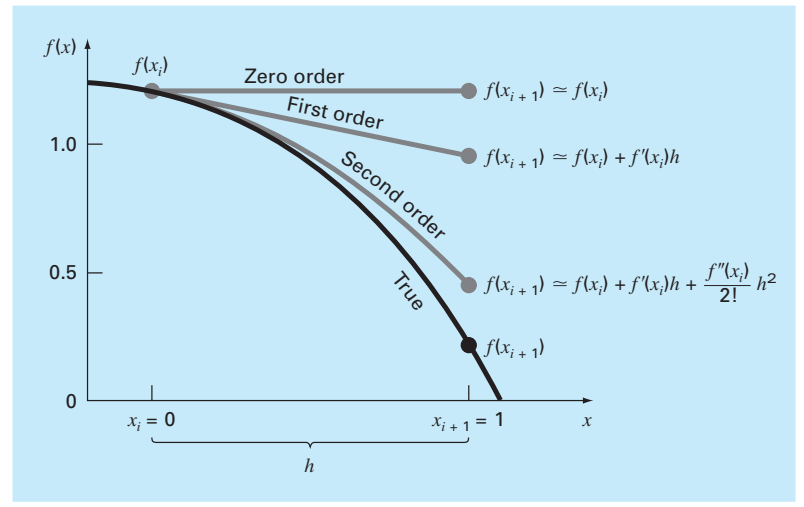
\includegraphics[height=0.6\textheight]{../chapra_7th/Chapra_Fig_4_1.png}
\par}
    
\end{frame}



\begin{frame}
\fontsize{9}{10}\selectfont

\begin{block}{Chapra Contoh 4.2}
Gunakan deret Taylor dengan $n=0$ sampai $n=6$ untuk mengaproksimasi
fungsi $f(x) = \cos(x)$ pada $x_{i+1} = \pi/3$ dengan titik referensi
$x_{i} = \pi/4$.
\end{block}

Untuk kasus ini $h=x_{i+1} - x_{i} = \pi/3 - \pi/4 = \pi/12$.
Hasil dapat dilihat pada tabel berikut.

{\centering
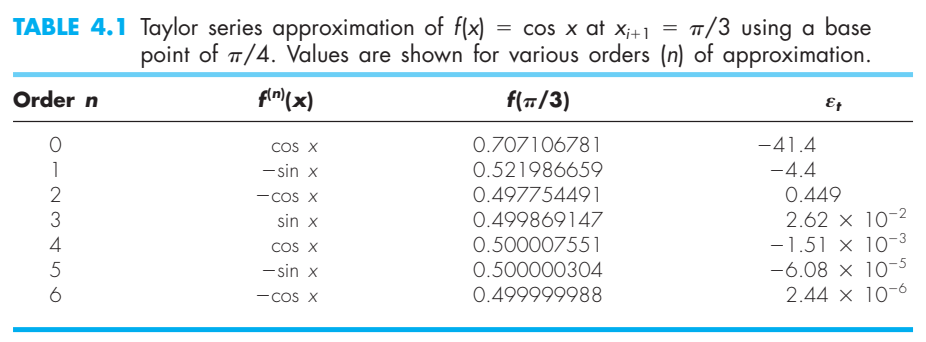
\includegraphics[height=0.5\textheight]{../chapra_7th/Chapra_Table_Example_4_2.png}
\par}

\end{frame}


\begin{frame}{Deret Taylor dan Aproksimasi}
\fontsize{9}{10}\selectfont

Secara umum, deret Taylor dengan $n$-suku akan eksak untuk polinomial
orde-$n$. Untuk fungsi lain yang diferensiabel dan kontinu, seperti eksponensial
dan sinusoid, diperlukan jumlah suku deret yang tak-hingga agar eksak.

Dalam banyak kasus, penggunaan jumlah suku yang berhingga akan menghasilkan
aproksimasi yang cukup dekat dengan nilai sebenarnya. Seberapa banyak suku
yang diperlukan agar dapat menghasilkan aproksimasi yang cukup baik bergantung
dari suku sisa $R_{n}$ dari ekspansi.

Ada beberapa hal yang perlu diingat mengenai suku sisa dari deret Taylor.
Perhatikan bahwa $\xi$ tidak diketahui, selain dari syarat bahwa $\xi$ terletak
di antara $x_{i}$ dan $x_{i+1}$. Kedua, untuk menentukan turunan ke-$n+1$ dari
$f(x)$, tentu saja kita harus mengetahui $f(x)$. Akan tetapi, jika $f(x)$ diketahui
kita tidak perlu menggunakan deret Taylor, kita cukup menggunakan $f(x)$.

Meskipun tidak dapat digunakan secara praktis, Persamaan suku sisa masih
berguna untuk memberikan gambaran mengenai galat pemotongan yang terjadi.
Hal ini karena kita dapat mengatur suku yang terkait dengan $h$ pada ekspansi
deret Taylor: kita dapat memiliki sejauh mana dari $x$ kita ingin mengevaluasi $f(x)$
dan jumlah suku yang ingin kita perhitungkan.
\end{frame}



\begin{frame}{Estimasi galat pemotongan}
Persamaan suku sisa biasanya dinyatakan dengan:
$$
R_{n} = \mathcal{O}(h^{n+1})
$$
yang berarti bahwa galat pemotongan yang terjadi memiliki orde $h^{n+1}$. Hal ini
berguna untuk \textit{perbandingan} dalam estimasi galat pemotongan.

Misalnya jika sisa atau galat pada deret Taylor adalah $\mathcal{O}(h)$, maka
jika ukuran langkah $h \rightarrow h/2$ maka galat $\epsilon \rightarrow \epsilon/2$. 

Pada kasus lain, jika galat deret Taylor adalah $\mathcal{O}(h^2)$ maka
jika ukuran langkah $h \rightarrow h/2$ maka galat $\epsilon \rightarrow \epsilon/4$.

\end{frame}